\tikzset{every picture/.style={line width=0.75pt}} %set default line width to 0.75pt        

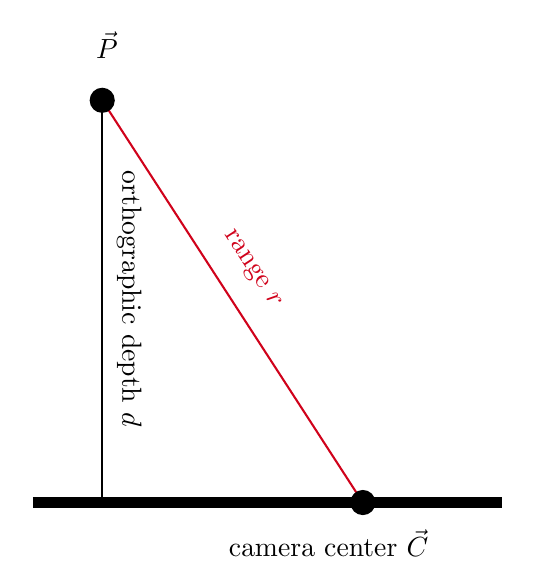
\begin{tikzpicture}[x=0.75pt,y=0.75pt,yscale=-1,xscale=1]
%uncomment if require: \path (0,273); %set diagram left start at 0, and has height of 273

%Straight Lines [id:da7423207506186664] 
\draw [line width=3.75]    (17.08,234.29) -- (243.08,234.29) ;
%Straight Lines [id:da2664879119929795] 
\draw    (50.5,40.5) -- (50.5,234.92) ;
%Straight Lines [id:da2932541940464021] 
\draw [color={rgb, 255:red, 208; green, 2; blue, 27 }  ,draw opacity=1 ]   (50.5,40.5) -- (176.08,234.29) ;
%Shape: Circle [id:dp5274939901831479] 
\draw  [draw opacity=0][fill={rgb, 255:red, 0; green, 0; blue, 0 }  ,fill opacity=1 ] (170.02,234.29) .. controls (170.02,230.94) and (172.74,228.23) .. (176.08,228.23) .. controls (179.43,228.23) and (182.15,230.94) .. (182.15,234.29) .. controls (182.15,237.64) and (179.43,240.35) .. (176.08,240.35) .. controls (172.74,240.35) and (170.02,237.64) .. (170.02,234.29) -- cycle ;
%Shape: Circle [id:dp5178837685841811] 
\draw  [draw opacity=0][fill={rgb, 255:red, 0; green, 0; blue, 0 }  ,fill opacity=1 ] (44.44,40.5) .. controls (44.44,37.15) and (47.15,34.44) .. (50.5,34.44) .. controls (53.85,34.44) and (56.56,37.15) .. (56.56,40.5) .. controls (56.56,43.85) and (53.85,46.56) .. (50.5,46.56) .. controls (47.15,46.56) and (44.44,43.85) .. (44.44,40.5) -- cycle ;

% Text Node
\draw (114.53,100) node [anchor=north west][inner sep=0.75pt]  [color={rgb, 255:red, 208; green, 2; blue, 27 }  ,opacity=1 ,rotate=-56.88] [align=left] {range $\displaystyle r$};
% Text Node
\draw (71,73) node [anchor=north west][inner sep=0.75pt]  [rotate=-90] [align=left] {orthographic depth $\displaystyle d$};
% Text Node
\draw (110,246) node [anchor=north west][inner sep=0.75pt]  [color={rgb, 255:red, 0; green, 0; blue, 0 }  ,opacity=1 ] [align=left] {camera center $\displaystyle \vec{C}$};
% Text Node
\draw (46,6) node [anchor=north west][inner sep=0.75pt]   [align=left] {$\displaystyle \vec{P}$};


\end{tikzpicture}

